\documentclass[11pt]{beamer}
\usetheme{Madrid}
\usepackage[utf8]{inputenc}
\usepackage{amsmath}

\usepackage{tikz}
\usetikzlibrary{calc}
\usepackage{svg}

\author[\texttt{sebastiano.tronto@uni.lu}]{Sebastiano Tronto}
\title[Python Intro and a bit of Sage]%
{A Practical Introduction to Python (and a bit of Sage)}
\logo{
\includegraphics[scale=0.1]{img/unilu.jpg}} 
%\institute{University of Luxembourg} 

\date{2021-04-02} 

\begin{document}

\begin{frame}
  \titlepage
\end{frame}

\begin{frame}{Second part - schedule}
  \begin{tabular}{l|c|c|l}
    \textbf{Date} & \textbf{Topics} & \textbf{Homework} & \textbf{Deadline}  \\
    \hline
    April 2   & Python ``review'', a bit of Sage & (see March 26) & April 18 \\
    \hline
    April 23  & Sage: Algebra and Crypto & Homework 3 & May 9                \\
    \hline
    May 7     & Sage: Analysis and Statistics  & Homework 4 & May 30         \\
    \hline
    May 21    & Fast code, other software  &
  \end{tabular}
\end{frame}


\begin{frame}{What is programming?}
  \begin{columns}
    \column{0.35\textwidth}
      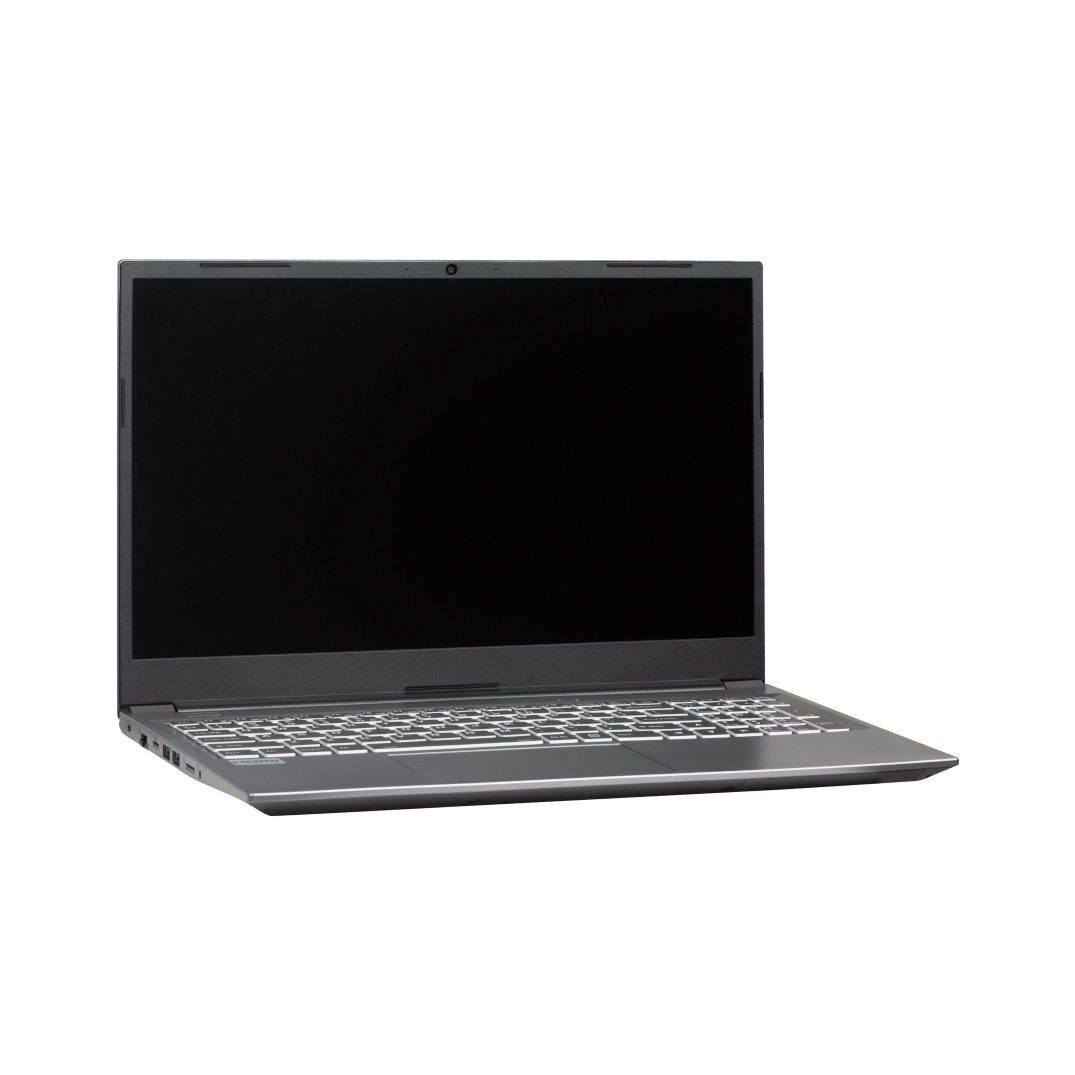
\includegraphics[scale=0.12]{img/laptop.png}
    \column{0.1\textwidth}
      \begin{center}
\includegraphics[scale=0.12]{img/equal.png}\end{center}
    \column{0.35\textwidth}
      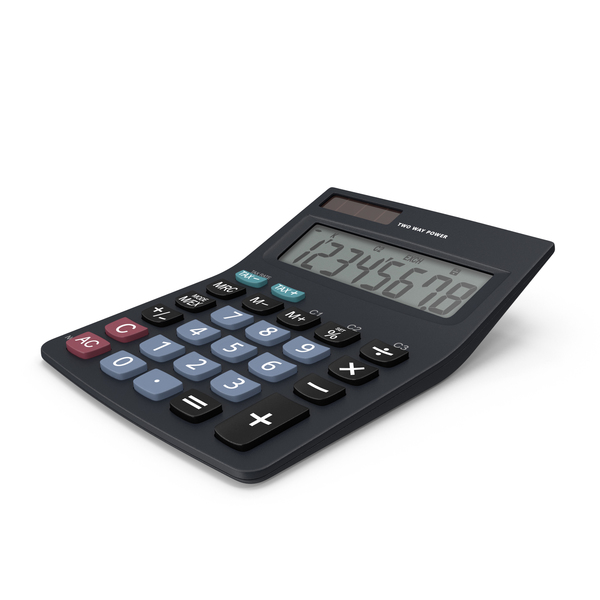
\includegraphics[scale=0.9]{img/calc.jpg}
  \end{columns}
  \begin{itemize}
    \item Software (apps): commands written in a \emph{programming language}
    \item Programming language: mix of English and symbols
    \item The code is \emph{compiled} to machine language (C, C++) or\\
          \emph{interpreted} by some software in the middle (Python)
  \end{itemize}
\end{frame}


\begin{frame}{Python}
  \begin{columns}
    \column{0.7\textwidth}
      \url{https://www.python.org}

      \vspace{0.3cm}
      \begin{itemize}
        \item Interpreted: slower than C, usable interactively
        \item Simple syntax, easy to learn
        \item Very popular
        \item Sage is based on Python
      \end{itemize}
    \column{0.25\textwidth}
      
\includegraphics[scale=0.16]{img/python.png}
  \end{columns}
\end{frame}

\begin{frame}{The interpreter - Python as a calculator}
  \begin{center}
    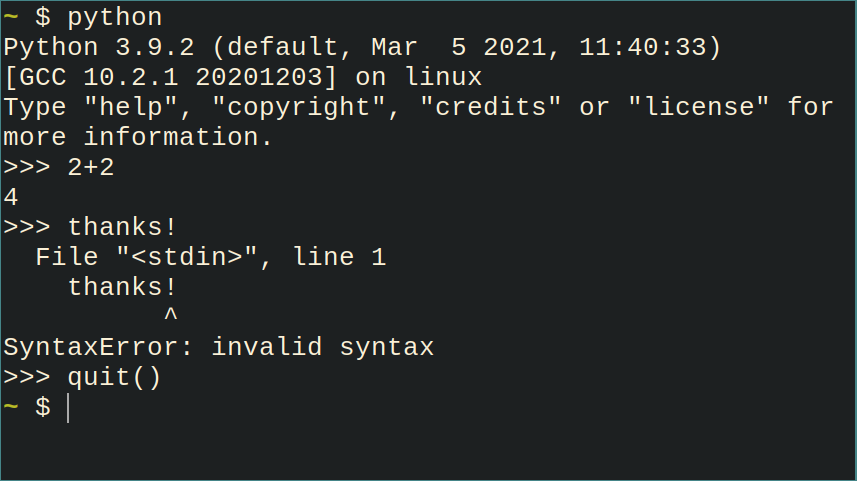
\includegraphics[scale=0.3]{img/term.png}
  \end{center}
\end{frame}

\begin{frame}{The interpreter - Python as a calculator}
  \url{https://www.python.org/shell}

  \vspace{0.3cm}
  \begin{itemize}
    \item Each line executed as you enter it, result is printed
    \item Usual math operations work: try them!
      \begin{center}
        \texttt{a+b, a-b, a*b, a/b}\\
        \texttt{a**b (power), a//b (integer division), a\%b (remainder)}
      \end{center}
    \item More math functions:
      \begin{center} \begin{tabular}{l}
        \texttt{import math} \\
        \texttt{math.sqrt(3)}
      \end{tabular} \end{center}
  \end{itemize}
\end{frame}


\begin{frame}{Help!}
  \begin{itemize}
    \item Type \texttt{help()} for interactive help
    \item Try \texttt{help("math")} and \texttt{help("import")}
    \item What does
      \begin{center} \texttt{from math import *} \end{center}
    do?
  \end{itemize}
\end{frame}

\begin{frame}{Variables}
  \texttt{variable\_name = value \qquad \# This is an assignment}

  \vspace{0.3cm}
  \begin{itemize}
    \item Save results, use them later
    \item \texttt{variable\_name}: combination of letters, numbers, underscores
    \item \texttt{=} always means \emph{assignment}, never \emph{equality}
  \end{itemize}
\end{frame}

\begin{frame}{Types}
  \texttt{type(variable\_name) \qquad \# Get the type of a variable}

  \vspace{0.3cm}
  \begin{itemize}
    %\item Tells the computer how to read a variable
    \item In other languages you must specify the type of a variable
    \item Python figures out automatically (\emph{dynamic typing})
    \item Each type allows different operations
  \end{itemize}
\end{frame}


\begin{frame}{Other types: Boolean and String}
  \texttt{my\_bool = True}

  \texttt{s1 = "hello!" \qquad \# Same as 'hello!'}

  \vspace{0.3cm}
  \begin{itemize}
    \item \texttt{bool}: \texttt{True} or \texttt{False}
      \begin{itemize}
        \item Operations on \texttt{bool}:
              \texttt{and}, \texttt{or}, \texttt{not}
        \item Operations with boolean result: \texttt{==}, \texttt{!=},
              \texttt{>}, \texttt{<}, \texttt{>=}, \texttt{<=}
      \end{itemize}
    \item \texttt{str}: a string of characters
      \begin{itemize}
        \item Useful operations:

          \begin{tabular}{ll}
            \texttt{len({\bf str})} & \texttt{\# Length, integer value}   \\
            \texttt{{\bf str} + {\bf str}} & \texttt{\# Concatenation} \\
            \texttt{{\bf int} * {\bf str}} & \texttt{\# Repetition}
          \end{tabular}
      \end{itemize}
  \end{itemize}
\end{frame}

\begin{frame}{Lists and sets}
  %\texttt{(2.5, True, "hello") \qquad \# Tuple}

  \texttt{[2.5, True, "hello"] \qquad \# List}

  \texttt{\{2.5, True, "hello"\} \qquad \# Set}

  \vspace{0.3cm}
  \begin{itemize}
    %\item Different collections of objects
    %\item Tuple: immutable
    \item Lists: keep order and duplicates
    \item Sets: disregard order and duplicates, allow set operations
  \end{itemize}
\end{frame}


\begin{frame}{Lists and sets}
  Things in common (\emph{\texttt{A} is a list or a set}):

  \vspace{0.3cm}
  \begin{itemize}
    \item \texttt{len(A)}: number of elements (\texttt{\bf int})
    \item \texttt{x in A}: check if \texttt{x} is in \texttt{A}
          (\texttt{\bf bool})
    \item If \texttt{A} contains numbers: \texttt{max(A)}, \texttt{min(A)},
          \texttt{sum(A)}
  \end{itemize}

  \vspace{0.3cm}
  Pass from one type to the other: \texttt{set(A)} and \texttt{list(A)}
\end{frame}

\begin{frame}{List (and set) comprehension}
  \texttt{[x**2 {\bf for} x {\bf in} [-1,4,1,0] {\bf if} x < 3]
          \quad\# Result: [1,1,0]}

  \texttt{\{x**2 {\bf for} x {\bf in} [-1,4,1,0] {\bf if} x < 3\}
          \quad\# Result: \{0,1\}}

  \vspace{0.3cm}
  \begin{itemize}
    \item Mathematical way to define lists and sets
    \item Complete syntax:

          \vspace{0.2cm}
          \texttt{[f(x,y,\dots) {\bf for} x {\bf in} L {\bf for} y {\bf in} M
                   \dots \quad {\bf if} cond(x,y,\dots)]}

          \vspace{0.2cm}
          \begin{itemize}
            \item Use as many variables \texttt{x, y, \dots} as you want
            \item \texttt{L, M, \dots} are lists or sets or other collections
            \item \texttt{f(x,y,\dots)} is any expression depending on the
                  variables
            \item \texttt{cond(x,y,\dots)} has Boolean value
          \end{itemize}
  \end{itemize}
\end{frame}

\begin{frame}{Lists: access elements and sublists}
  \begin{tabular}{ll}
    \texttt{A[i]} &
    \texttt{\# i-th element of A ($i\in \{0,\dots,\texttt{len(A)}-1\}$)} \\
    \texttt{A[i] = value} & \texttt{\# Change i-th element of A} \\
    \texttt{A[i:j:k]} & \texttt{\# Sublist from A[i] to A[j] with step k} \\
    \texttt{A[i:j]} & \texttt{\# Same as A[i:j:1]} \\
    \texttt{A[i:]} & \texttt{\# Same as A[i:len(A):1]} \\
    \texttt{A[:j]} & \texttt{\# Same as A[0:j:1]}
  \end{tabular}
\end{frame}

\begin{frame}{List operations}
  \begin{tabular}{ll}
    \texttt{A.append(x)} & \texttt{\# Append x to A ({\bf change A})} \\
    \texttt{A.insert(i,x)} &
    \texttt{\# Insert x in position i ({\bf change A})} \\
    \texttt{del A[i]} & \texttt{\# Remove i-th element of A ({\bf change A})}\\
  \end{tabular}

  \vspace{1cm}
  \begin{tabular}{ll}
    \texttt{A+B} & \texttt{\# Concatenation of A and B ({\bf list})} \\
    \texttt{A*n} & \texttt{\# Repetition of A ({\bf list})} \\
  \end{tabular}
\end{frame}

\begin{frame}{Set operations}
  \begin{tabular}{ll}
    \texttt{A.add(x)} & \texttt{\# Add x to A ({\bf change A})} \\
    \texttt{A.remove(x)} & \texttt{\# Remove x from A ({\bf change A})}\\
  \end{tabular}

  \vspace{0.5cm}
  \begin{tabular}{ll}
    \texttt{A < B} (or \texttt{A <= B}) &
    \texttt{\# A contained in (or equal to) B ({\bf bool})} \\
    \texttt{A > B} (or \texttt{A >= B}) &
    \texttt{\# A containes (or is equal to) B ({\bf bool})} \\
  \end{tabular}

  \vspace{0.5cm}
  \begin{tabular}{ll}
    \texttt{A | B} & \texttt{\# Union ({\bf set})} \\
    \texttt{A \& B} & \texttt{\# Intersection ({\bf set})}\\
    \texttt{A - B} & \texttt{\# Set difference ({\bf set})} \\
  \end{tabular}
\end{frame}

\begin{frame}{Writing more complex programs}
  \begin{center}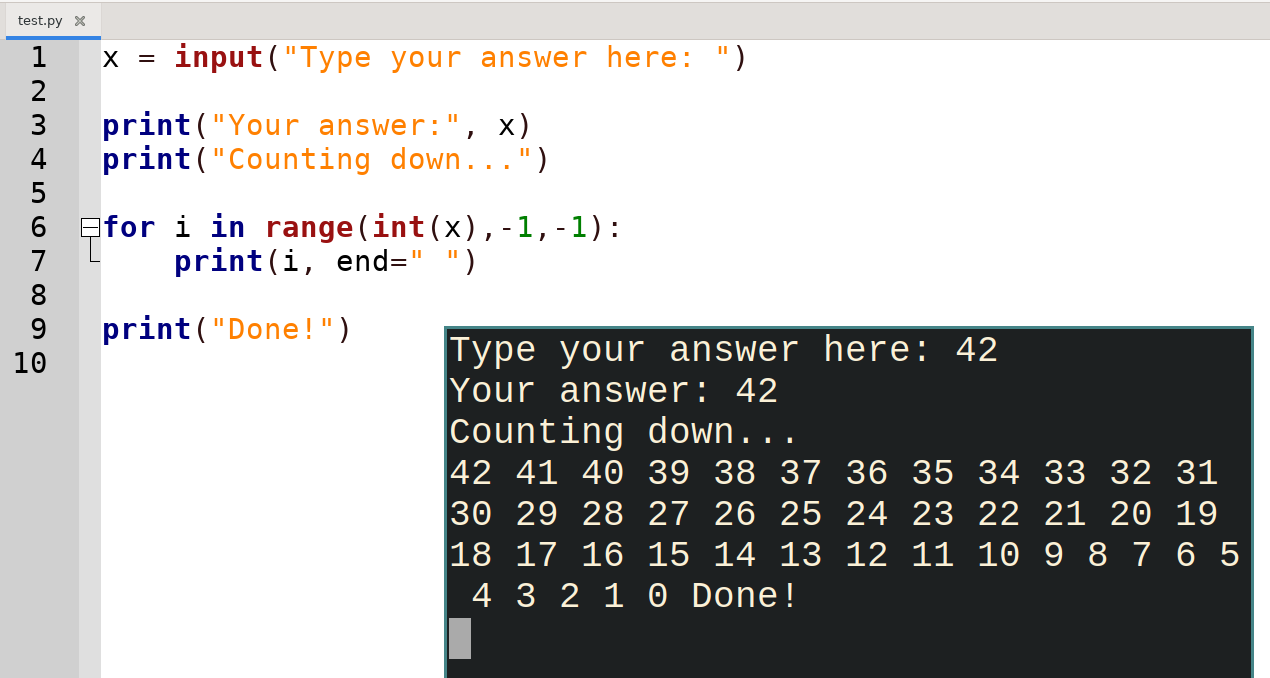
\includegraphics[scale=0.25]{img/geany.png}\end{center}
\end{frame}

\begin{frame}{Non-interactive Python}
  \begin{itemize}
    \item You can write a file (for example with \url{https://www.geany.org})
    \item Output results with \texttt{print("string", or, other, values)}
    \item Get input (\texttt{str}) with \texttt{x = input("Prompt: ")},
          convert with \texttt{int(x)} or \texttt{float(x)}\dots
    \item Blocks of code: use \emph{indentation} (see next slides)
  \end{itemize}
\end{frame}

\begin{frame}[fragile]{\texttt{if} statement}
  \begin{columns}
    \column{0.45\textwidth}
      \texttt{{\bf if} \emph{condition}:}

      \texttt{\qquad instruction1}
      
      \texttt{\qquad instruction2}

      \texttt{\qquad \dots}

      \texttt{{\bf else}: \# This is optional}

      \texttt{\qquad other inst}
    \column{0.55\textwidth}
      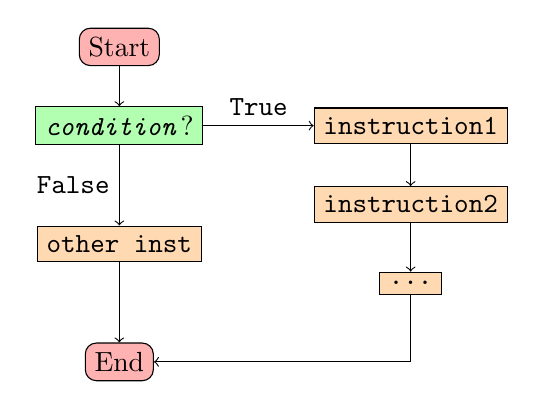
\begin{tikzpicture}
        \tikzstyle{s} = [rectangle, rounded corners, text centered,
                                                       draw=black, fill=red!30]
        \tikzstyle{p} = [rectangle, text centered, draw=black, fill=orange!30]
        \tikzstyle{d} = [rectangle, text centered, draw=black, fill=green!30]

        \node(start)  [s]                     {Start};
        \node(cond)   [d, below of=start]     {\texttt{\emph{condition}}?};
        \node(inst1)  [p, right of=cond, xshift=2.7cm] {\texttt{instruction1}};
        \node(inst2)  [p, below of=inst1]     {\texttt{instruction2}};
        \node(dots)   [p, below of=inst2]     {\texttt{\dots}};
        \node(other)  [p, below of=cond, yshift=-0.5cm]  {\texttt{other inst}};
        \node(end)    [s, below of=other, yshift=-0.5cm] {End};

        \draw[->] (start) -- (cond);
        \draw[->] (cond) -- node[anchor=south] {\texttt{True}} (inst1);
        \draw[->] (inst1) -- (inst2);
        \draw[->] (inst2) -- (dots);
        \draw[->] (cond) -- node[anchor=east] {\texttt{False}} (other);
        \draw[->] (dots) |- (end);
        \draw[->] (other) -- (end);
      \end{tikzpicture}
  \end{columns}
\end{frame}


\begin{frame}[fragile]{\texttt{while} loop}
  \begin{columns}
    \column{0.45\textwidth}
      \texttt{{\bf while} \emph{condition}:}

      \texttt{\qquad instruction1}
      
      \texttt{\qquad instruction2}

      \texttt{\qquad \dots}
    \column{0.55\textwidth}
      \begin{tikzpicture}
        \tikzstyle{s} = [rectangle, rounded corners, text centered,
                                                       draw=black, fill=red!30]
        \tikzstyle{p} = [rectangle, text centered, draw=black, fill=orange!30]
        \tikzstyle{d} = [rectangle, text centered, draw=black, fill=green!30]

        \node(start)  [s]                     {Start};
        \node(cond)   [d, below of=start]     {\texttt{\emph{condition}}?};
        \node(inst1)  [p, right of=cond, xshift=2.7cm] {\texttt{instruction1}};
        \node(inst2)  [p, below of=inst1]     {\texttt{instruction2}};
        \node(dots)   [p, below of=inst2]     {\texttt{\dots}};
        \node(end)    [s, below of=other, yshift=-0.5cm] {End};

        \draw[->] (start) -- (cond);
        \draw[->] (cond) -- node[anchor=south] {\texttt{True}} (inst1);
        \draw[->] (inst1) -- (inst2);
        \draw[->] (inst2) -- (dots);
        \draw[->] (cond) -- node[anchor=east] {\texttt{False}} (end);
        \draw[->] (dots) -| ($(cond.south)+(0.4,0)$);
      \end{tikzpicture}
  \end{columns}
\end{frame}

\begin{frame}{\texttt{for} loop}
  \texttt{{\bf for} i {\bf in} A:}

  \texttt{\qquad instruction1}
  
  \texttt{\qquad instruction2}

  \texttt{\qquad \dots}

  \vspace{0.3cm}
  \begin{itemize}
    \item Repeats instructions as \texttt{i} varies in \texttt{A}
    \item \texttt{A} can be list, set or other collection
    \item Example: \texttt{A} can be \texttt{range(\emph{a,b,step})}
  \end{itemize}
\end{frame}


\begin{frame}{Functions}
  \texttt{{\bf def} f(x, y, \dots): }

  \texttt{\qquad instruction1}
  
  \texttt{\qquad instruction2}

  \texttt{\qquad \dots}

  \texttt{\qquad {\bf return} some\_value}

  \vspace{0.3cm}
  \begin{itemize}
    \item Useful to divide programs into ``pieces''
    \item The result of \texttt{f(x,y,\dots)} is given by \texttt{return \dots}
  \end{itemize}
\end{frame}

\begin{frame}{An example of function (with recursion)}
  \texttt{def fibonacci(n):}

  \texttt{\qquad if n == 0:}

  \texttt{\qquad \qquad return 0}

  \texttt{\qquad if n == 1:}

  \texttt{\qquad \qquad return 1}

  \texttt{\qquad return fibonacci(n-1) + fibonacci(n-2)}

  \vspace{0.3cm}
  \begin{itemize}
    \item Elegant, but slow (in this case)
    \item Can get stuck in infinite loop: when?
  \end{itemize}
\end{frame}

\begin{frame}{Sage}
  \begin{center}
    \includesvg[scale=0.5]{img/sage}

    \url{https://www.sagemath.org}
  \end{center}

  \vspace{0.3cm}
  \begin{itemize}
    \item Mathematical software, uses Python as a language
    \item Use it interactively or with Jupyter notebook
    \item Try it online: \url{https://sagecell.sagemath.org} or
          \url{https://cocalc.com/app}
  \end{itemize}
\end{frame}

\begin{frame}{Differences with Python}
  \begin{tabular}{l|l}
    \textbf{Python} & \textbf{Sage}                                          \\
    \texttt{{\color{gray}>>>} {\color{blue}type(5)}} &
    \texttt{{\color{gray}sage:} {\color{blue}type(5)}}                       \\
    \texttt{<class 'int'>} & \texttt{<class 'sage.rings.integer.Integer'>}   \\
    \texttt{{\color{gray}>>>} {\color{blue}5/2}} &
    \texttt{{\color{gray}sage:} {\color{blue}5/2}}                           \\
    \texttt{2.5} & \texttt{5/2}                                              \\
    \texttt{{\color{gray}>>>} {\color{blue}type(5/2)}} &
    \texttt{{\color{gray}sage:} {\color{blue}type(5/2)}}                     \\
    \texttt{<class 'float'>} &
    \texttt{<class 'sage.rings.rational.Rational'>}                          \\
    \texttt{{\color{gray}>>>} {\color{blue}type(2.5)}} &
    \texttt{{\color{gray}sage:} {\color{blue}type(2.5)}}                     \\
    \texttt{<class 'float'>} &
    \texttt{<class 'sage.rings.real\_mpfr.RealLiteral'>}                     \\
    \texttt{{\color{gray}>>>} {\color{blue}5**3}} &
    \texttt{{\color{gray}sage:} {\color{blue}5\^{}3}}                        \\
    \texttt{125} & \texttt{125}
  \end{tabular}
\end{frame}

\begin{frame}{Sage Documentation}
  \begin{itemize}
    \item Tutorial (guided examples): type \texttt{tutorial()} or visit
          \url{https://doc.sagemath.org/html/en/tutorial}
    \item \texttt{help()}: works as in Python
    \item Reference manual (detailed technical information):
          \url{https://doc.sagemath.org/html/en/reference}
  \end{itemize}
\end{frame}


\end{document}

